\documentclass[a4paper, 12pt]{article}
\usepackage[T2A]{fontenc}
\usepackage[utf8]{inputenc}
\usepackage[english,russian]{babel}
\usepackage{amsmath, amsfonts, amssymb, amsthm, mathtools, misccorr, indentfirst, multirow}
\usepackage{wrapfig}
\usepackage{graphicx}
\usepackage{subfig}
\usepackage{adjustbox}
\usepackage{pgfplots}

\usepackage{geometry}
\geometry{top=20mm}
\geometry{bottom=20mm}
\geometry{left=20mm}
\geometry{right=20mm}
\newcommand{\angstrom}{\textup{\AA}}

\title{Лабораторная работа № 4.3.3\\Исследование разрешающей способности микроскопа методом Аббе.}
\author{Нехаев Александр. гр. 654}
\date{\today}

\begin{document}
	\maketitle
	\newpage
	\tableofcontents
	\newpage
	\section{Введение}
	\paragraph{Цель работы:} изучение дифракционного предела разрешения объектива микроскопа.
	\paragraph{В работе используются:} лазер; кассета с набором сеток разного периода; линзы; щель с микрометрическим винтом; оптический стол с набором рейтеров и крепежных винтов; экран; линейка.\par
	Всякая оптическая система, предназначенная для получения изображений, имеет конечный предел разрешения, т.е. ограниченную возможность раздельного наблюдения близких частей предмета. Принципиальной причиной, ограничивающей предел разрешения, является дифракция световых волн: ограничение пучка лучей краями линз и диафрагм, составляющих оптическую систему, приводит к нарушению \textit{стигматричности} изображения — каждая точка предмета отображается не в одну точку, а в дифракционное пятно. Дифракционные пятна от близких точек предмета могут перекрываться друг другом, в результате чего точки становятся неразличимыми.\par
	\textit{Разрешающей способностью оптического прибора} называется минимальное расстояние $l_{\min}$ между двумя точками в пространстве предметов, изображения которых разрешаются по критерию Релея.\par
	Природа дифракционных искажения общая для всех оптических систем; мы рассмотрим для примера глаз, лупу и простейший объектив микроскопа, состоящий из одной линзы (разрешение оптических приборов определяется обычно дифракцией на объективе).\par
	Оценим разрешающую способность глаза, полагая, что предмет (рис. \ref{fig:1}) расположен на расстоянии наилучшего зрения $L=25$ см от зрачка диаметром $d_0=5$ мм. Согласно критерию Релея глаз различает изображение точек как два объекта, если угловое расстояние между точками соответствует угловому размеру дифракционного пятна:
	\begin{wrapfigure}{1}{6cm}
		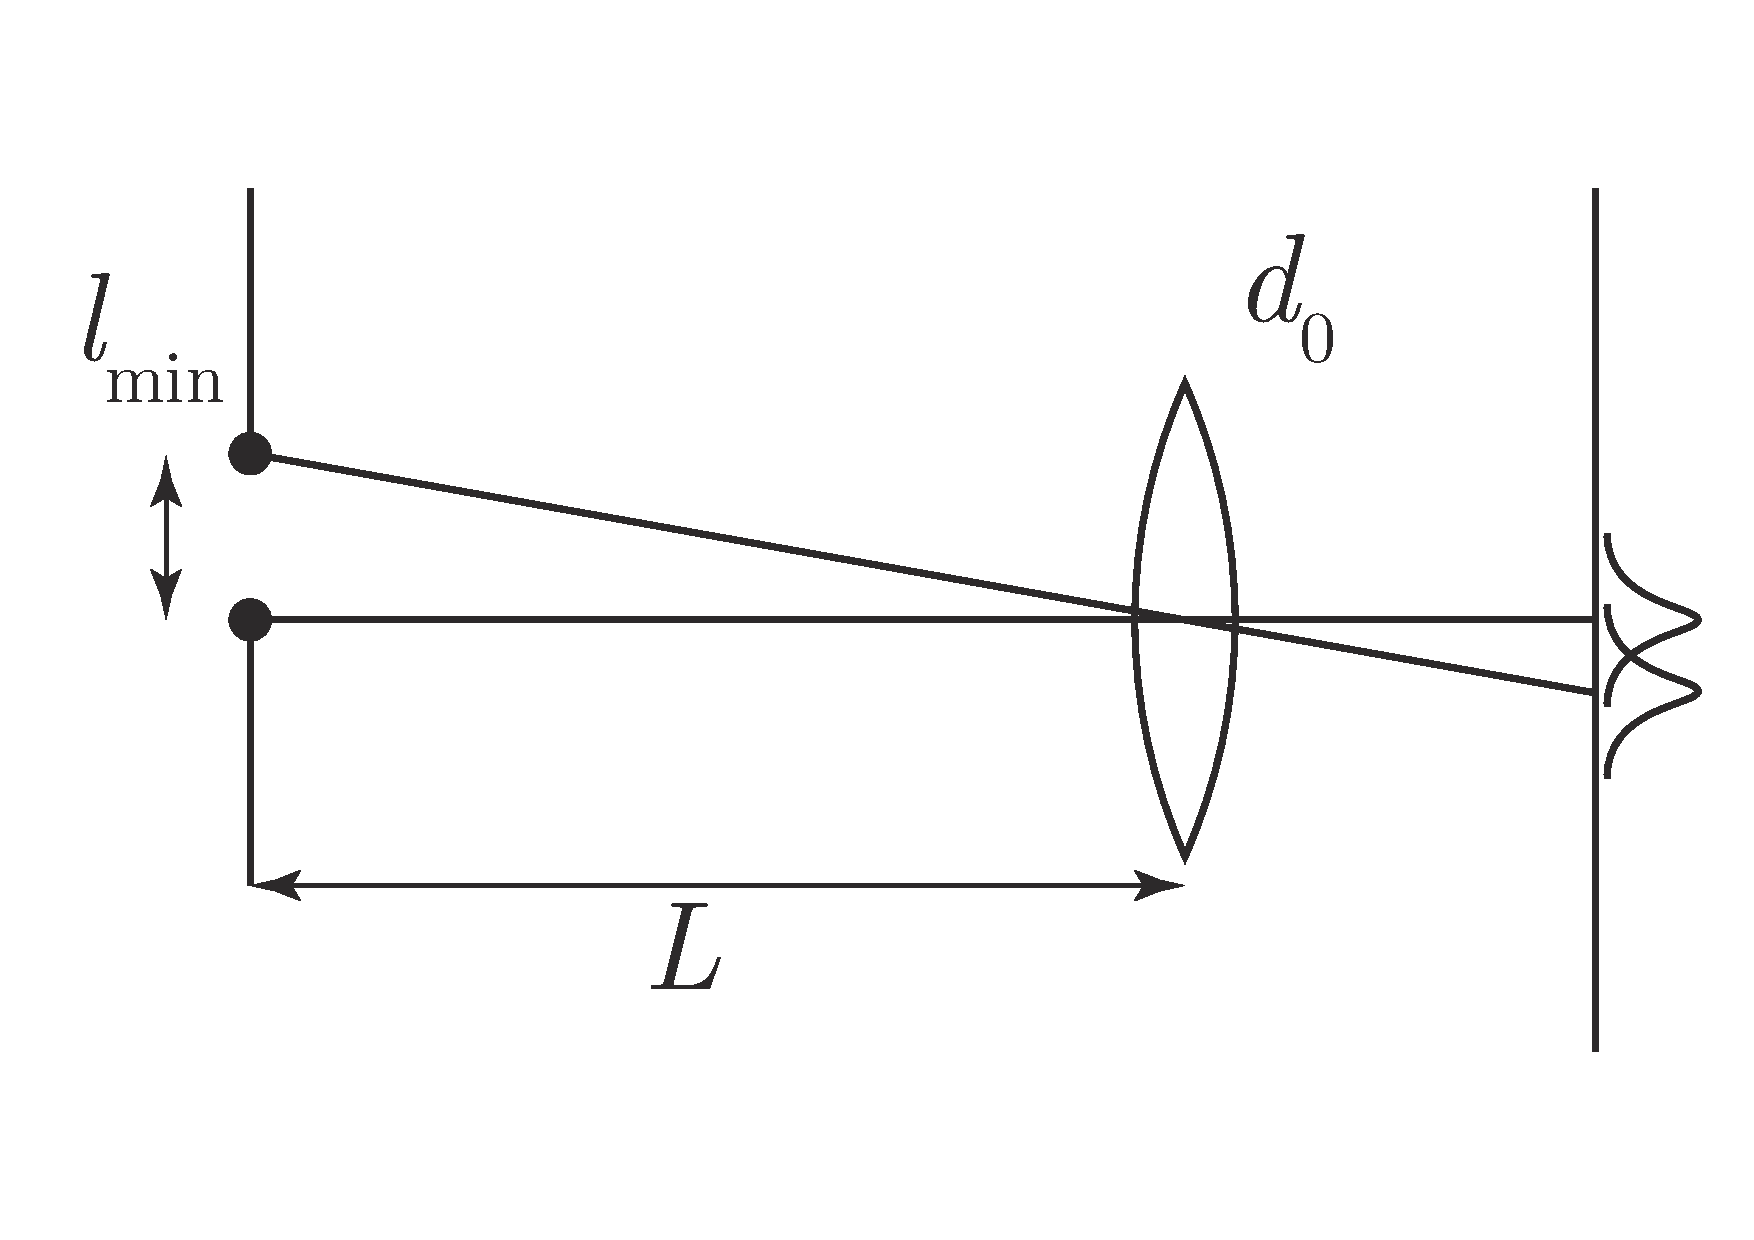
\includegraphics[scale=0.2]{fig1.pdf}
		\caption{Разрешающая способность глаза}
		\label{fig:1}
	\end{wrapfigure}
	\begin{equation*}
		\frac{l_{\min}}{L}=\frac{\lambda}{d_0}\quad\text{или}\quad l_{\min}=\lambda\frac{L}{d_0}\approx\lambda\frac{25}{0.5}\approx 50\lambda.
	\end{equation*}
	Для $\lambda\approx 6000$ \AA расчёт дает $l_{\min}\approx 30$ мкм.\par
	Для лупы диаметром $D_0$ с фокусным расстоянием $f$ при настройке глаза на бесконечность
	\begin{equation*}
		l_{\min}=\lambda\frac{f}{D_0}.
	\end{equation*}\par
	Для иммерсионного микроскопа (объект находится в иммерсионной среде — жидкости с показателем преломления $n$) разрешающая способность объектива
	\begin{equation*}
		l_{\min}\approx\frac{0.61\lambda}{n\sin u}\approx \frac{\lambda}{2n\sin u},
	\end{equation*}
	где $u$ — апертурный угол объектива микроскопа (см. рис. \ref{fig:2}), т.е. угол между оптической осью и лучом, направленным из центра объекта в край линзы (напомним, что при наблюдении в микроскоп объект занимает небольшой участок, располагающийся вблизи оптической оси объектива).\par
	Если наблюдения с помощью микроскопа ведутся при внешнем освещении, то, как правило, различные точки предмета рассеивают когерентные волны. Теория разрешающей способности для случая освещаемых объектов была разработана Аббе.\par
	Схема образования изображения в объектива микроскопа представлена на рис. \ref{fig:2}. Для простоты рассмотрим случай, когда предметом является периодическая структура (дифракционная решетка), освещаемая параллельным пучком лучей. При наблюдении в микроскоп предмет располагается вблизи переднего фокуса объектива\par
	\begin{figure}
		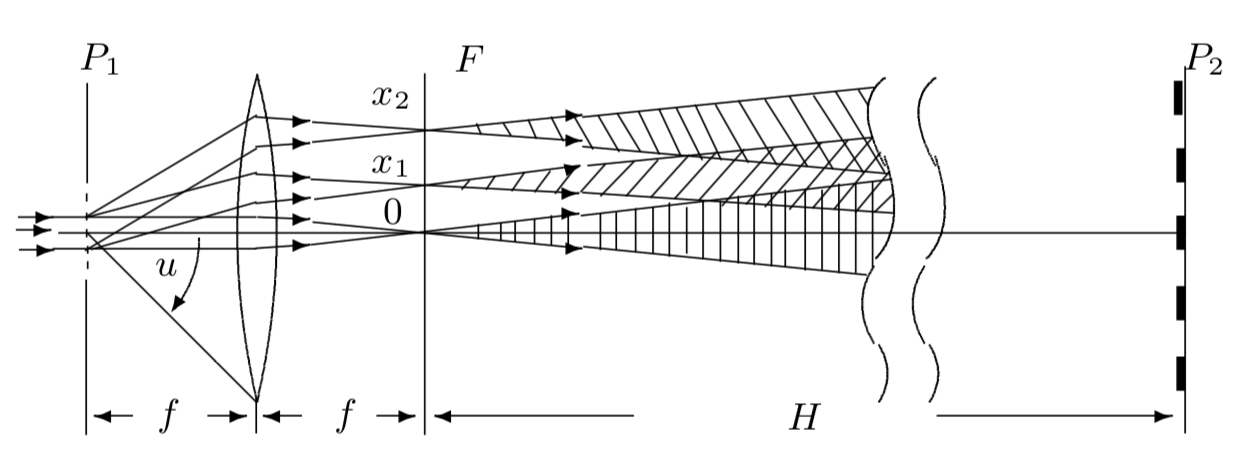
\includegraphics[scale=0.4]{fig2.png}
		\caption{Образование изображения в объективе микросокпа. $P_1$ — плоскость предмета, $F$ — задняя фокальная плоскость объектива, $P_2$ — плоскость, сопряженная с предметной плоскостью. В плоскости $P_2$ световые пучки сильно перекрываются.}
		\label{fig:2}
	\end{figure}
	Аббе предложил иной подход к оценке разрешающей способности: прохождение лучей от предмета к изображению разбивается на два этапа. Сначала рассматривается картина, возникающая в задней фокальной плоскости $F$ объектива. Эта картина называется \textit{первичным изображением} или \textit{фурье-образом} предмета. Затем первичное изображение рассматривается как источник волн, создающих изображением предмета в плоскости $P_2$, сопряженной плоскости предмета, т.е. \textit{вторичное изображение}. Такой подход основан на \textit{принципе Гюйгенса-Френеля}, согласно которому любой участок волнового фронта можно рассматривать как вторичный источник излучения.\par
	Легко понять, что первичное изображение, наблюдаемое в задней фокальной плоскости объектива, представляет собой картину дифракции Фраунгофера на объекте (в нашем случае — на дифракционной решетке). Действительно, на решетку падает плоская волна, а каждая точка наблюдения в фокальной плоскости $F$ линзы соответствует бесконечно удаленной точке. Смещение $x_{\min}$ точки наблюдения от оптической оси связано с углом наклона $\varphi_m$ параллельного пучка лучей перед линзой соотношением (при малых $\varphi$): $x_m\approx f\varphi_m$.\par
	\begin{figure}
		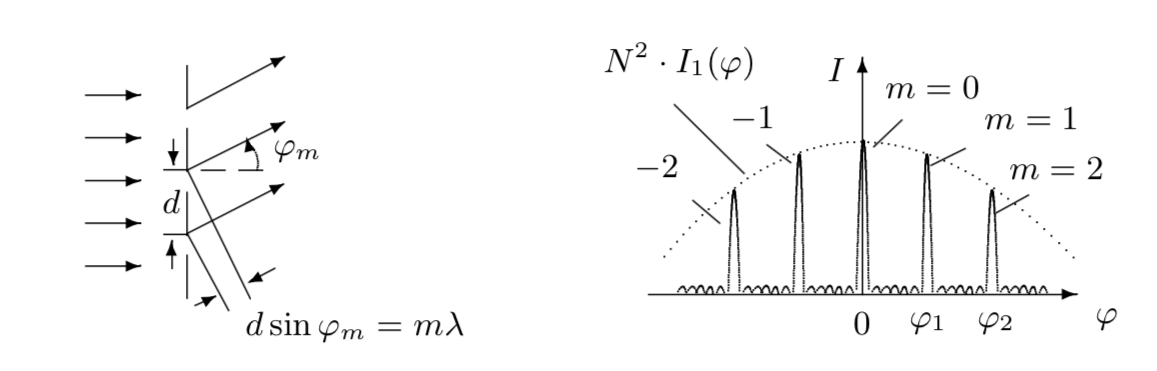
\includegraphics[scale=0.4]{fig3.png}
		\caption{Спектр амплитудной решетки. $I_1\left(\varphi\right)$ — распределение интенсивности при дифракции света на одиночной щели, $N$ — число щелей решетки.}
		\label{fig:3}
	\end{figure}
	При дифракции Фраунгофера на одномерной решетке периода $d$ направления $\varphi_m$ максимальной интенсивности (главные максимумы) определяются условием:
	\begin{equation}
		d\sin\varphi_m=m\lambda
		\label{eq:1}
	\end{equation}
	где $\lambda$ — длина световой волна. Главные максимумы различных порядков $m$ имеют неодинаковые интенсивности (рис. \ref{fig:3}). Таким образом, первичное изображение представляет собой набор ярких точек, расположенных цепочкой на равных расстояниях друг от друга. Излучение этих когерентных точечных источников создаст в плоскости $P_2$ систему интерференционных полос, синтезирующих изображение предмета (решетки) в этой плоскости.\par
	При таком рассмотрении дифракционные искажения, обусловленные конечным диаметром линзы, связаны с тем, что часть первичного изображения закрывается. Через микроскоп проходят только те пучки, для которых выполняется условие
	\begin{equation}
		\varphi_m<u,
	\end{equation}
	где $u$ — \textit{апертурный угол} (рис. \ref{fig:2}). Эти пучки лучей собираются в задней фокальной плоскости линзы, так что за ней возникают расходящиеся пучки лучей с центрами в плоскости $F$. В плоскости $P_2$ эти пучки интерферируют и воспроизводят увеличенное изображение решетки.\par
	Из рис. \ref{fig:2} ясно, что диафрагмы практически одинаковых размеров, расположенные в фокальной плоскости $F$ или непосредственно на объективе, перекрывают те же самые пучки лучей. Таким образом, дифракцию на оправе объективе в рассмотрении Аббе можно заменить дифракцией на диафрагме $D$, равной по размеру диаметру работающей (открытой) части линзы и расположенной в задней фокальной плоскости $F$.\par
	Рассмотрим вначале крайний случай, когда через диафрагму в плоскости $F$ проходит только один максимум — максимум нулевого прядка. Картина в $P_2$ изображает при этом объект, первичное изображение которого сводится к одному центральному максимуму. Но такая картина возникает лишь в том случае, когда параллельный пучок не претерпевает никакой дифракции, т. е. если решетка вообще отсутствует; в плоскости $P_2$ получается поэтому равномерное распределение освещенности и решетка не видна.\par
	Если приоткрыть диафрагму и поставить её несимметрично, так, чтобы прошел только нулевой и один из первых максимумов, то на экране получится изображение, имеющее вид периодической структуры с плавным переходом от светлых мест к темным; такое изображение характерно для двухлучевой интерференции. Рассчитаем период изображения в плоскости $P_2$ для этого случая. Линейное расстояние $x_1$ между максимумами нулевого и первого порядка в плоскости $F$ есть
	\begin{equation}
		x_1\approx f\varphi=f\lambda/d.
	\end{equation}
	Ширина $l$ интерференционных полос, образующихся в плоскости $P_2$, может быть найдена по формуле
	\begin{equation}
		l=\lambda/\omega,
	\end{equation}
	где $\omega=x_1/H$ — угол схождения интерферирующих лучей в точке наблюдения, расположенной в плоскости $P_2$, а $H$ — расстояние между плоскостями $F$ и $P_2$. Таким образом,
	\begin{equation}
		l\approx\lambda H/x_1=Hd/f.
	\end{equation}
	Согласно геометрической оптике изображение решетки в плоскости $P_2$ должно иметь период
	\begin{equation}
		d'\approx\frac{H+f}{f}d.
	\end{equation}
	\begin{wrapfigure}{1}{6cm}
		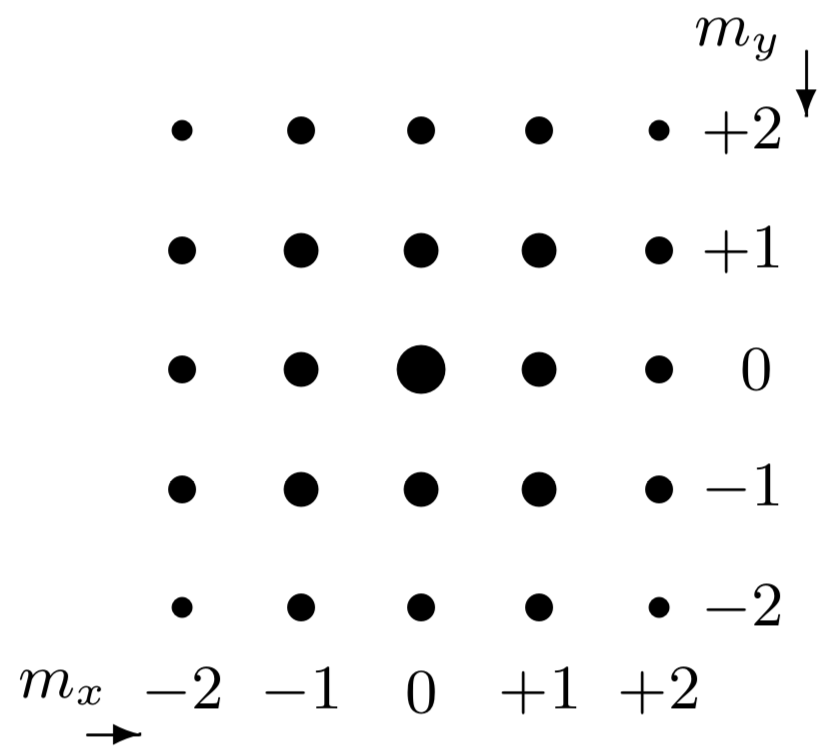
\includegraphics[scale=0.2]{fig4.png}
		\caption{Дифракция Фраунгофера на двумерной решетке (сетке). Максимумы изображены кружками, размеры которых характеризуют интенсивности.}
		\label{fig:4}
	\end{wrapfigure}
	Поскольку в случае микроскопа предмет располагается вблизи передней фокальной плоскости объектива, и, следовательно $H\gg f$, получаем: $l\approx d'$. Таким образом, с помощью дифракционных максимумов нулевого и первого порядка в увеличенном масштабе передается основной период решетки (и не воспроизводятся никакие детали структуры, например, наличие резкой границы между светлыми и темными участками дифракционной решетки).\par
	Если задержать каким-либо образом в плоскости $F$ максимум первого порядка, а вместо него пропустить максимум второго порядка, то в $P_2$ возникает система полос с периодом в два раза меньшим, так что на экране будто видно изображение более частой решетки, чем имеющаяся в действительности. Максимумы высших порядков создает более узкие интерференционные полосы, они ответственны за передачу более тонких деталей.\par
	Из изложенного ясно, что для получения правильного изображения надо, чтобы через объектив микроскопа проходили дифракционные пучки разных напралвений. Как уже отмечалось ранее, если апертурный угол $u$ меньше $\varphi_1$, то в плоскости $P_2$ не возникает периодического изображения. Соотношение
	\begin{equation}
		\sin u\geqslant\lambda/d
	\end{equation}
	можно рассматривать как условие разрешения решетки с периодом $d$. Отсюда можно найти минимальное разрешаемое объективом расстояник
	\begin{equation}
		d\geqslant\frac{\lambda}{\sin u}\approx\frac{\lambda}{D/2f}.
		\label{eq:8}
	\end{equation}
	При этом диафрагма $D$, расположенная симметрично, пропускает нулевой и $\pm 1$ максимумы.\par
	При освещении решетки пучками, наклонными к оси, когда через диафрагму, кроме нулевого, проходит всего один из двух первых максимумов (этого достаточно для изображения периодической структуры без тонких деталей), условие разрешения принимает вид
	\begin{equation*}
		d\geqslant\frac{\lambda}{2\sin u}.
	\end{equation*}\par
	В нашей работе применяется двумерная решетка сетка. Ее можно рассматривать как две скрещенные (перпендикулярные друг к другу) решетки. Узкий пучок монохроматического света, пройдя через решетку с вертикальными штрихами, дает совокупность максимумов, расположенных вдоль горизонтальной линии. Световой пучок, соответствующий каждому максимуму, проходя через вторую решетку, распадается на новую совокупность световых пучков, дающих максимумы вдоль вертикальной линии. Главные максимумы возникают тогда, когда одновременно выполняются условия:
	\begin{equation}
		d\sin\varphi_x=m_x\lambda,\quad d\sin\varphi_y=m_y\lambda,
	\end{equation}
	где $m_x$ и $m_y$ — целые числа, характеризующие порядки дифракционных максимумов, $\varphi_x$ и $\varphi_y$ — направления на главные дифракционные максимумы в горизонтальной и вертикальной плоскостях соответственно.\par
	Максимумы, удовлетворяющие условию $\varphi_x, \varphi_y<u$, создают в задней фокальной плоскости $F$ объектива картину дифракции Фраунгофера (рис. \ref{fig:4}) – первичное изображение.\par
	Если теперь поместить в фокальной плоскости вертикальную щель так, чтобы через нее проходили дифракционные максимумы с $m_x=0$ и $m_y=0,\pm1,\pm2,...,$ то в плоскости $P_2$ получается изображение решетки с горизонтально расположенными штрихами. Если, наоборот, пропустить максимумы с $m_y=0$ и $m_x=0,\pm1,\pm2,...,$ то в $P_2$ получится изображение решетки с вертикальными штрихами. Таким образом можно продемонстрировать явление \textit{пространственной фильтрации} — выделение различных структур в изображении.
	\section{Экспериментальная установка}
	Схема модели проекционного микроскопа приведена на рис. \ref{scheme}. Предметом служат сетки, расположенные в кассете. Смена сеток осуществляется поворотом внешнего кольца кассеты.\par
	\begin{figure}[h]
		\centering
		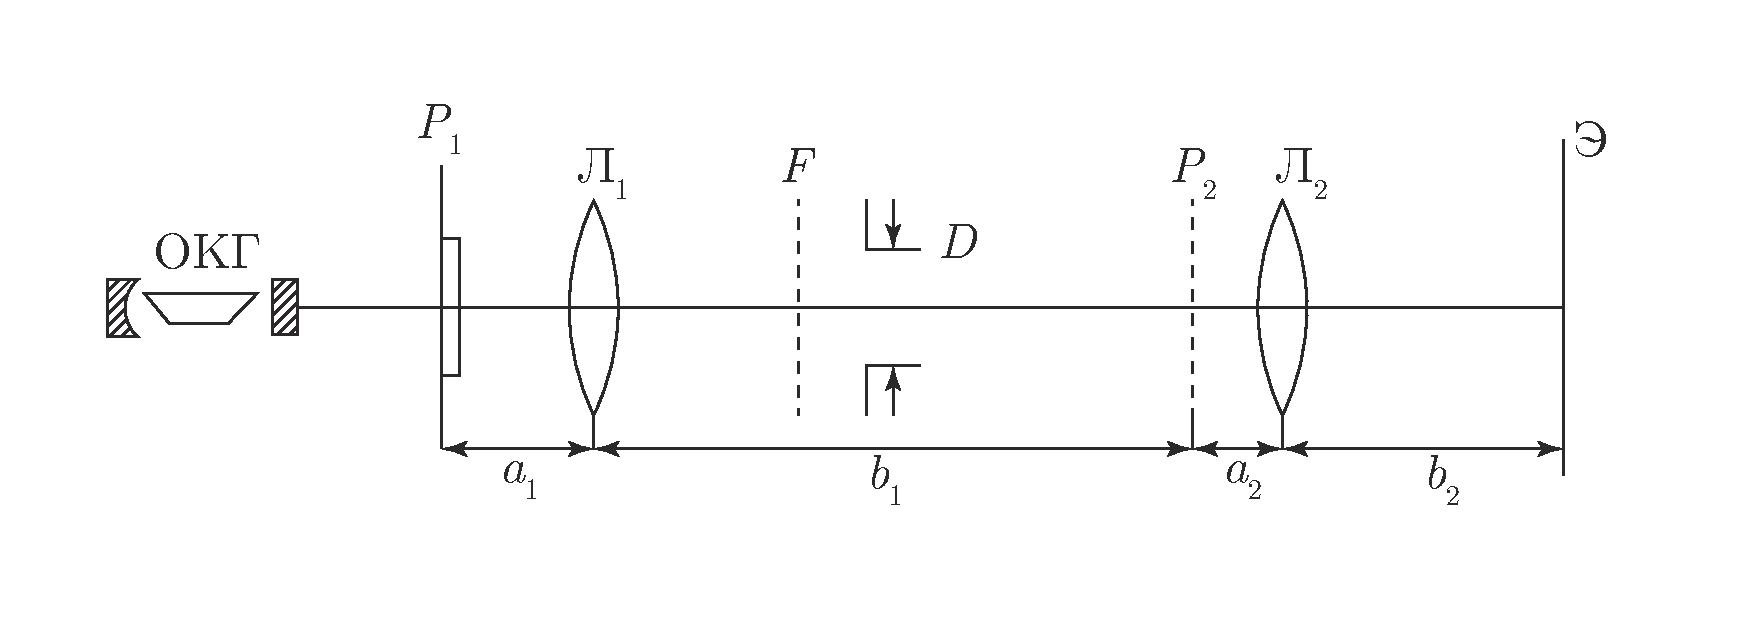
\includegraphics[scale=0.6]{scheme.pdf}
		\caption{Схема экспериментальной установки — модель проекционного микроскопа}
		\label{scheme}
	\end{figure}
	Излучение лазера (ОКГ) почти перпендикулярно падает на сетку $\text{C}$, установленную вблизи фокальной плоскости линзы $\text{Л}_1$ — объектива микроскопа. Обычно и объектив и окуляр микроскопа — короткофокусные линзы (1-3 см). В нашей модели линза $\text{Л}_1$ выбирается достаточно длиннофокусной ($f\approx 10$ см), т.к. размер первичного изображения в фокальной плоскости $F$ должен быть не слишком малыми, чтобы дополнительными диафрагмами можно было влиять на вторичное изображение в плоскости $P_2$. Вторичное изображение из плоскости $P_2$ проецируется на экран $\text{Э}$ линзой $\text{Л}_2$ (короткофокусной, чтобы изображение на экране было крупнее). Во избежание микротравм глаза от излучения лазера не следует использовать эту линзу традиционным образом как окуляр микроскопа.\par
	Изображение сетки периодически повторяется — \textit{репродуцируется} – в пространстве между сеткой и первой линзой, поэтому для того, чтобы среди множества репродуцированных изображений сетки можно было выделить её гармоническое изображение, на одну из сеток наложена  тонкая проволочка, т.е. непериодический объект, изображена которого не репродуцируется.\par
	В фокальной плоскости $F$ могут быть установлены диафрагмы — щелевая или ирисовая (отверстие с переменным диаметром) и различного рода маски (препятствия).\par
	Как видно из соотношения (\ref{eq:8}), минимально разрешимый шаг решетки или сетки определяется апертурным углом $u$ объектива. Обычно апертура микроскопа меняется с помощью ирисовой диафрагмы на объективе (на линзе $\text{Л}_1$ такая диафграгма есть), но в наших условиях удобнее располагать щелевую диафрагму в плоскости $F$. Имея набор сеток с различными периодами $d$ и изменяя апертурный угол объектива с помощью щелевой диафрагмы, можно экспериментально проверить соотношение (\ref{eq:8}).\par
	В нашей работе период сеток рассчитывается двумя способами: в первом способе (дифракция Фраунгофера) — расстояние между дифракционными максимумами на экране измеряется при помощи линейки, а затем по формуле решетки (\ref{eq:1}) определяется её период; во втором способе период определяется по увеличенному с помощью модели микроскопа изображению сетки на экрана.\par
	С помощью откалиброванных таким образом сеток определяется разрешающая способоность микроскопа. Для этого в задней фокальной плоскости $F$ объектива устанавливается щелевая диафрагма с микрометрическим винтом и подбирается её минимальный размер, при котором еще видно изображение сетки на экране (щель пропускает максимумы с $m=0,\text{ }\pm1$). По размеру диафрагмы и фокусному расстоянию объектива рассчитывается апертурный угол $u$ и проверяется соотношение (\ref{eq:8}).\par
	Для выполнения последней части работы ширина вспомогательной щели и угол наклона к оси системы подбираются так, чтобы на экране вместо изображения сетки получалось изображение решётки, расположенной наклонно, т.е. осуществлялась \textit{пространственная фильтрация}. Если сетку и щель поменять местами, то соответствующим подбором сетки можно <<рассечь>> первичное изображение так, что изображение щели на экране будут многократно повторяться — мультиплицироваться.
	\section{Ход работы}
	\subsection{Определение периода решеток по их пространственному спектру}
	Для измерения расстояния между соседними дифракционными максимумами(в нашем случае вертикальными) и число промежутков между ними. Измерим расстояние $L=120$ см. Длина волны лазера $\lambda=532$ нм. $n$ — кол-во точек между которыми отмеряем расстояние. $m$ — расстояние между точками в сантиметрах.
	\begin{equation*}
		\sin\varphi=\tan\varphi\approx h/b
	\end{equation*}
	где $h$ — расстояние между максимумами, а $b$ — расстояние до экрана. Используя формулу главных максимумов имеем:
	\begin{table}[h]
	\centering
	\begin{tabular}{|c|c|c|c|c|}
  		\hline
  		$n$ & $m$, см & $h$ & $\sin\varphi$ & $d$, нм\\
  		\hline
  		3 & 10.3 & 3.43(3) & 0.028611111 & 18.8038835\\
  		6 & 6.6 & 1.1 & 0.009166667 & 58.69090909\\
  		6 & 6,9 & 1,15 & 0,009583333	 & 56,13913043\\
  		12 & 6,9 & 0,575 & 0,004791667 & 112,2782609\\
  		24 & 10,5 & 0,4375 & 0,003645833 & 147,5657143\\
  		\hline
	\end{tabular}
	\end{table}
	\subsection{Определение периода решеток по изображению увеличенной модели микроскопа}
	Создав модель микроскопа, мы можем получить изображение самой решётки на экране.\par
	Измерим период увеличенного изображения решётки. Для нахождения периода решётки необходимо разделить полученный период изображения на увеличение Г.
\\
	Линза 1: $f=10$ см.\\
	Линза 2: $f=25\text{мм}=2.5$ см.\\
	\\
	$a_1=11 \text{см}\pm 0.1 \text{см}$\\
	$a_2=f_2=2.5\text{см}\pm 0.1\text{см}$\\
	$b_1=66\text{см}\pm 2\text{см}$\\
	$b_2=58\text{см}\pm 2\text{см}$\\
	Длинна <<тубуса>> микроскопа $(a_2+b_1)=60.5$ см.\\
	Увеличение для системы линз $\Gamma=\frac{b_1b_2}{a_1+a_2}=\frac{66\cdot58}{11+2.5}=112$.\\
	Периоды изображений сеток на экране:
	\begin{table}[h]
		\centering
		\begin{tabular}{|c|c|c|}
			\hline
			№ решетки & $h_1$, мм & $d$, мкм\\
			\hline
			1 & 2 & 14.15\\
			2 & 4 & 34.16\\
			3 & 9 & 55.7\\
			4 & 12 & 114.24\\
			5 & 18 & 160.87\\
			\hline
		\end{tabular}
	\end{table}
	\subsection{Определение периода решеток по оценке разрешающей способности микроскопа}
	Определяем минимальный размер диафрагмы при котором изображение решетки(сетки). При меньших размерах щели изображение выглядит как одномерная решетка). Для решетки 1  картина не получается четкой даже при самом большом расширении щели.\\
	$D=f(2)=5\pm0,1$ мм\\
	$D=f(3)=3,9\pm0,1$ мм\\
	$D=f(4)=2,9\pm0,1$ мм\\
	$D=f(5)=1,9\pm0,1$ мм\\
	\begin{equation*}
		l_{\min}\approx\frac{\lambda}{D/\left(2f\right)},
	\end{equation*}
	где $f$ — фокусное расстояние $\text{Л}_1$.
	\begin{table}[h]
		\centering
		\begin{tabular}{|c|c|c|}
			\hline
			№ решетки& $D$, мм & $l_{\min}$, мм\\
			\hline
			5 & 1.9 & 0.0023408\\
			4 & 2,9 & 0.002926\\
			3 & 3,9 & 0,003901333\\
			2 & 5 & 0,005852\\
			1 & $\emptyset$ & $\emptyset$\\
			\hline
		\end{tabular}
	\end{table}\par
	\newpage
	\begin{figure}
		\begin{tikzpicture}
			\begin{axis}[
				title={Зависимость $d=f\left(1/D\right)$},
				xlabel={$1/D$ (1/мкм)},
				ylabel={$d$, мкм},
				xmin=0,
				ymin=0,
				xmax=0.6,
				ymax=180,
				ymajorgrids=true,
   				xmajorgrids=true,
    			grid style=dashed,
    			width=\textwidth,
    			height=12cm,
			]
			\addplot+[
				color=black,
				mark=square,
				only marks,
				error bars/.cd,
				y dir=both, y explicit,
				x dir=both, x explicit
			]
			coordinates {
				(0.526315789,160.87)+-(0.031578947,12.8696)
				(0.344827586,114.24)+-(0.020689655,9.1392)
				(0.256410256,55.7)+-(0.015384615,4.456)
				(0.2,34.16)+-(0.012,2.7328)
			};
			\addplot[
				domain=0:0.6,
				samples=100,
				color=black,
			]
			{393.81*x-39.458};
			\end{axis}
		\end{tikzpicture}
	\end{figure}
	\section{Вывод}
	Используя данное оборудование, мы смогли определить период решёток и оценить разрешающую способность микроскопа.
\end{document}
